\documentclass{standalone}
\usepackage{tikz}
\usetikzlibrary{patterns, positioning}


\begin{document}
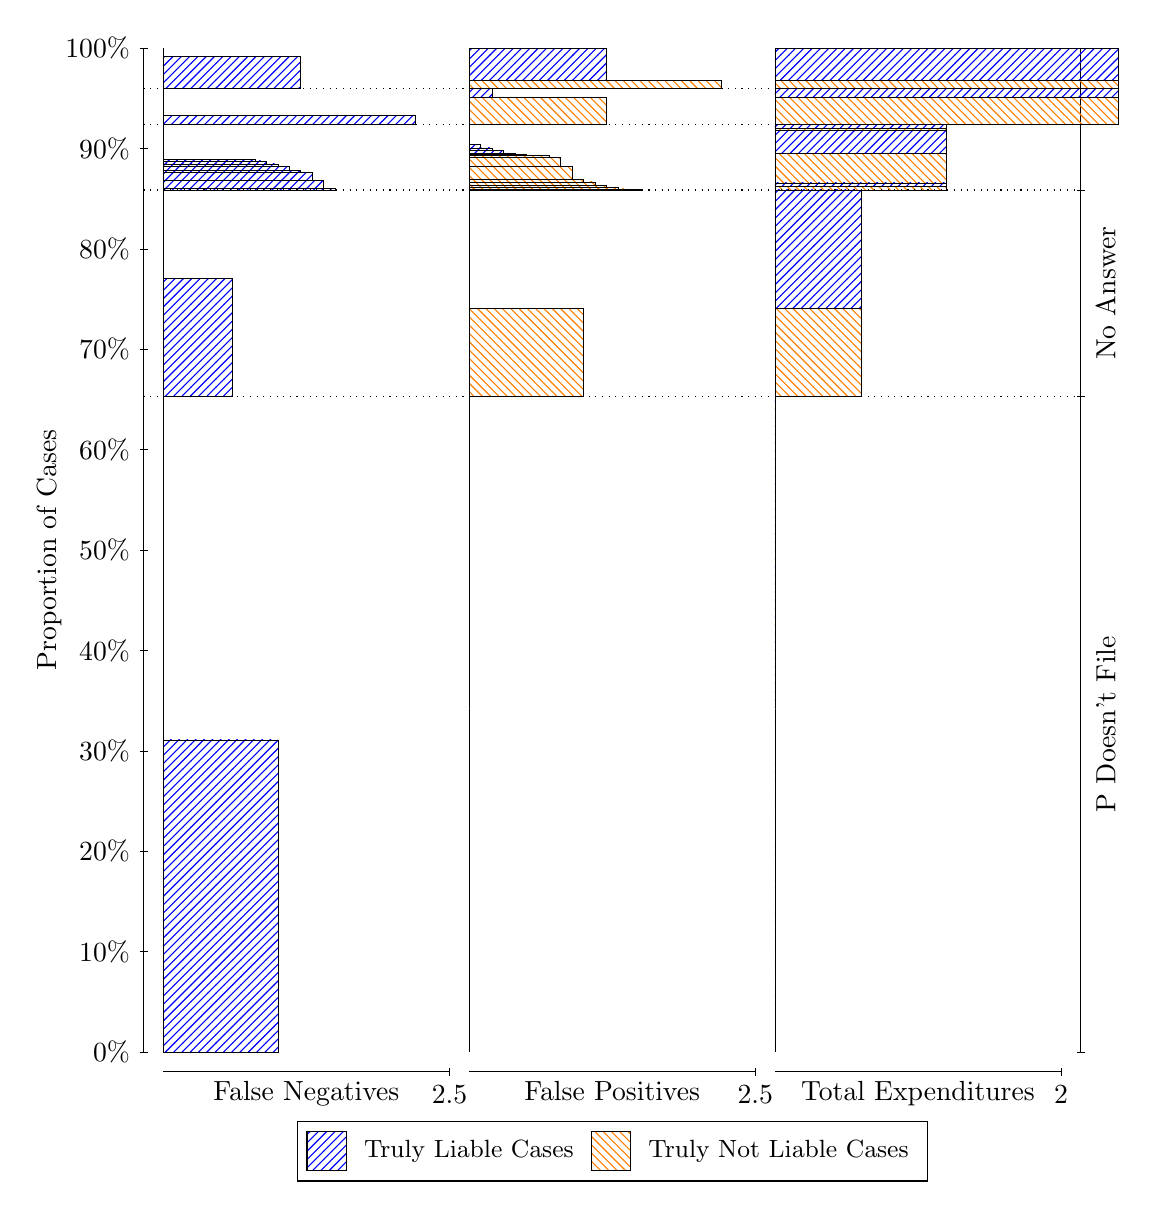
\begin{tikzpicture}
\draw[black, very thin] (1.5,1.75) -- (1.5,14.5);
\node[rotate=90, text=black, anchor=center] at (0.3, 8.125) {Proportion of Cases};
\draw[black, very thin] (1.45,1.75) -- (1.55,1.75);
\node[text=black, anchor=east] at (1.45, 1.75) {0\%};
\draw[black, very thin] (1.45,3.025) -- (1.55,3.025);
\node[text=black, anchor=east] at (1.45, 3.025) {10\%};
\draw[black, very thin] (1.45,4.3) -- (1.55,4.3);
\node[text=black, anchor=east] at (1.45, 4.3) {20\%};
\draw[black, very thin] (1.45,5.575) -- (1.55,5.575);
\node[text=black, anchor=east] at (1.45, 5.575) {30\%};
\draw[black, very thin] (1.45,6.85) -- (1.55,6.85);
\node[text=black, anchor=east] at (1.45, 6.85) {40\%};
\draw[black, very thin] (1.45,8.125) -- (1.55,8.125);
\node[text=black, anchor=east] at (1.45, 8.125) {50\%};
\draw[black, very thin] (1.45,9.4) -- (1.55,9.4);
\node[text=black, anchor=east] at (1.45, 9.4) {60\%};
\draw[black, very thin] (1.45,10.675) -- (1.55,10.675);
\node[text=black, anchor=east] at (1.45, 10.675) {70\%};
\draw[black, very thin] (1.45,11.95) -- (1.55,11.95);
\node[text=black, anchor=east] at (1.45, 11.95) {80\%};
\draw[black, very thin] (1.45,13.225) -- (1.55,13.225);
\node[text=black, anchor=east] at (1.45, 13.225) {90\%};
\draw[black, very thin] (1.45,14.5) -- (1.55,14.5);
\node[text=black, anchor=east] at (1.45, 14.5) {100\%};

\draw[black, very thin] (13.4,1.75) -- (13.4,14.5);
\draw[black, very thin] (13.35,1.75) -- (13.45,1.75);
\node[anchor=west] at (13.35, 1.75) {};
\draw[black, very thin] (13.35,10.076) -- (13.45,10.076);
\node[anchor=west] at (13.35, 10.076) {};
\draw[black, very thin] (13.35,12.697) -- (13.45,12.697);
\node[anchor=west] at (13.35, 12.697) {};
\draw[black, very thin] (13.35,13.531) -- (13.45,13.531);
\node[anchor=west] at (13.35, 13.531) {};
\draw[black, very thin] (13.35,13.984) -- (13.45,13.984);
\node[anchor=west] at (13.35, 13.984) {};
\draw[black, very thin] (13.35,14.5) -- (13.45,14.5);
\node[anchor=west] at (13.35, 14.5) {};

\draw[black, very thin, pattern color=blue, pattern=north east lines] (1.75,1.75) rectangle (3.2033,5.7139);
\draw[black, very thin, pattern color=orange, pattern=north west lines] (1.75,5.7139) rectangle (1.75,10.076);
\draw[black, very thin, pattern color=blue, pattern=north east lines] (1.75,10.076) rectangle (2.622,11.579);
\draw[black, very thin, pattern color=orange, pattern=north west lines] (1.75,11.579) rectangle (1.75,12.697);
\draw[black, very thin, pattern color=blue, pattern=north east lines] (1.75,12.697) rectangle (3.93,12.714);
\draw[black, very thin, pattern color=blue, pattern=north east lines] (1.75,12.714) rectangle (3.7847,12.82);
\draw[black, very thin, pattern color=blue, pattern=north east lines] (1.75,12.82) rectangle (3.6393,12.925);
\draw[black, very thin, pattern color=blue, pattern=north east lines] (1.75,12.925) rectangle (3.494,12.948);
\draw[black, very thin, pattern color=blue, pattern=north east lines] (1.75,12.948) rectangle (3.3487,12.996);
\draw[black, very thin, pattern color=blue, pattern=north east lines] (1.75,12.996) rectangle (3.2033,13.029);
\draw[black, very thin, pattern color=blue, pattern=north east lines] (1.75,13.029) rectangle (3.058,13.067);
\draw[black, very thin, pattern color=blue, pattern=north east lines] (1.75,13.067) rectangle (2.9127,13.081);
\draw[black, very thin, pattern color=blue, pattern=north east lines] (1.75,13.081) rectangle (2.7673,13.09);
\draw[black, very thin, pattern color=orange, pattern=north west lines] (1.75,13.09) rectangle (1.75,13.531);
\draw[black, very thin, pattern color=blue, pattern=north east lines] (1.75,13.531) rectangle (4.9473,13.64);
\draw[black, very thin, pattern color=orange, pattern=north west lines] (1.75,13.64) rectangle (1.75,13.984);
\draw[black, very thin, pattern color=blue, pattern=north east lines] (1.75,13.984) rectangle (3.494,14.391);
\draw[black, very thin, pattern color=orange, pattern=north west lines] (1.75,14.391) rectangle (1.75,14.5);
\draw[black, very thin, pattern color=orange, pattern=north west lines] (5.6333,1.75) rectangle (5.6333,6.1116);
\draw[black, very thin, pattern color=blue, pattern=north east lines] (5.6333,6.1116) rectangle (5.6333,10.076);
\draw[black, very thin, pattern color=orange, pattern=north west lines] (5.6333,10.076) rectangle (7.0867,11.194);
\draw[black, very thin, pattern color=blue, pattern=north east lines] (5.6333,11.194) rectangle (5.6333,12.697);
\draw[black, very thin, pattern color=orange, pattern=north west lines] (5.6333,12.697) rectangle (7.8133,12.704);
\draw[black, very thin, pattern color=orange, pattern=north west lines] (5.6333,12.704) rectangle (7.668,12.711);
\draw[black, very thin, pattern color=orange, pattern=north west lines] (5.6333,12.711) rectangle (7.5227,12.732);
\draw[black, very thin, pattern color=orange, pattern=north west lines] (5.6333,12.732) rectangle (7.3773,12.758);
\draw[black, very thin, pattern color=orange, pattern=north west lines] (5.6333,12.758) rectangle (7.232,12.799);
\draw[black, very thin, pattern color=orange, pattern=north west lines] (5.6333,12.799) rectangle (7.0867,12.827);
\draw[black, very thin, pattern color=orange, pattern=north west lines] (5.6333,12.827) rectangle (6.9413,12.995);
\draw[black, very thin, pattern color=orange, pattern=north west lines] (5.6333,12.995) rectangle (6.796,13.115);
\draw[black, very thin, pattern color=orange, pattern=north west lines] (5.6333,13.115) rectangle (6.6507,13.139);
\draw[black, very thin, pattern color=blue, pattern=north east lines] (5.6333,13.139) rectangle (6.36,13.147);
\draw[black, very thin, pattern color=blue, pattern=north east lines] (5.6333,13.147) rectangle (6.2147,13.162);
\draw[black, very thin, pattern color=blue, pattern=north east lines] (5.6333,13.162) rectangle (6.0693,13.2);
\draw[black, very thin, pattern color=blue, pattern=north east lines] (5.6333,13.2) rectangle (5.924,13.233);
\draw[black, very thin, pattern color=blue, pattern=north east lines] (5.6333,13.233) rectangle (5.7787,13.281);
\draw[black, very thin, pattern color=blue, pattern=north east lines] (5.6333,13.281) rectangle (5.6333,13.531);
\draw[black, very thin, pattern color=orange, pattern=north west lines] (5.6333,13.531) rectangle (7.3773,13.876);
\draw[black, very thin, pattern color=blue, pattern=north east lines] (5.6333,13.876) rectangle (5.924,13.984);
\draw[black, very thin, pattern color=orange, pattern=north west lines] (5.6333,13.984) rectangle (8.8307,14.093);
\draw[black, very thin, pattern color=blue, pattern=north east lines] (5.6333,14.093) rectangle (7.3773,14.5);
\draw[black, very thin, pattern color=orange, pattern=north west lines] (9.5167,1.75) rectangle (9.5167,6.1116);
\draw[black, very thin, pattern color=blue, pattern=north east lines] (9.5167,6.1116) rectangle (9.5167,10.076);
\draw[black, very thin, pattern color=orange, pattern=north west lines] (9.5167,10.076) rectangle (10.607,11.194);
\draw[black, very thin, pattern color=blue, pattern=north east lines] (9.5167,11.194) rectangle (10.607,12.697);
\draw[black, very thin, pattern color=orange, pattern=north west lines] (9.5167,12.697) rectangle (11.697,12.738);
\draw[black, very thin, pattern color=blue, pattern=north east lines] (9.5167,12.738) rectangle (11.697,12.786);
\draw[black, very thin, pattern color=orange, pattern=north west lines] (9.5167,12.786) rectangle (11.697,13.158);
\draw[black, very thin, pattern color=blue, pattern=north east lines] (9.5167,13.158) rectangle (11.697,13.451);
\draw[black, very thin, pattern color=orange, pattern=north west lines] (9.5167,13.451) rectangle (11.697,13.479);
\draw[black, very thin, pattern color=blue, pattern=north east lines] (9.5167,13.479) rectangle (11.697,13.531);
\draw[black, very thin, pattern color=orange, pattern=north west lines] (9.5167,13.531) rectangle (13.877,13.876);
\draw[black, very thin, pattern color=blue, pattern=north east lines] (9.5167,13.876) rectangle (13.877,13.984);
\draw[black, very thin, pattern color=orange, pattern=north west lines] (9.5167,13.984) rectangle (13.877,14.093);
\draw[black, very thin, pattern color=blue, pattern=north east lines] (9.5167,14.093) rectangle (13.877,14.5);
\draw[black, dotted] (1.5,10.076) -- (13.4,10.076);
\draw[black, dotted] (1.5,12.697) -- (13.4,12.697);
\draw[black, dotted] (1.5,13.531) -- (13.4,13.531);
\draw[black, dotted] (1.5,13.984) -- (13.4,13.984);
\draw[black, very thin] (1.75,1.5) -- (5.3833,1.5);
\node[text=black, anchor=north] at (3.5667, 1.5) {False Negatives};
\draw[black, very thin] (5.3833,1.45) -- (5.3833,1.55);
\node[text=black, anchor=north] at (5.3833, 1.45) {2.5};

\draw[black, very thin] (5.6333,1.5) -- (9.2667,1.5);
\node[text=black, anchor=north] at (7.45, 1.5) {False Positives};
\draw[black, very thin] (9.2667,1.45) -- (9.2667,1.55);
\node[text=black, anchor=north] at (9.2667, 1.45) {2.5};

\draw[black, very thin] (9.5167,1.5) -- (13.15,1.5);
\node[text=black, anchor=north] at (11.333, 1.5) {Total Expenditures};
\draw[black, very thin] (13.15,1.45) -- (13.15,1.55);
\node[text=black, anchor=north] at (13.15, 1.45) {2};

\node[text=black, centered, rotate=90] at (13.72, 5.9128) {P Doesn't File};
\node[text=black, centered, rotate=90] at (13.72, 11.386) {No Answer};




\draw (7.449999999999999,1.5) node[draw=none] (baseCoordinate) {};
\begin{scope}[align=center]
        \matrix[scale=0.5, draw=black, below=0.5cm of baseCoordinate, nodes={draw}, column sep=0.1cm]{
            \node[rectangle, draw, minimum width=0.5cm, minimum height=0.5cm, pattern color=blue, pattern=north east lines] {}; &
            \node[draw=none, font=\small, text=black] (B) {Truly Liable Cases}; &
            \node[rectangle, draw, minimum width=0.5cm, minimum height=0.5cm, pattern color=orange, pattern=north west lines] {}; &
            \node[draw=none, font=\small, text=black] (B) {Truly Not Liable Cases}; \\
            };
\end{scope}

\end{tikzpicture}
\end{document}